
\vspace{-.25in}
\subsection{Parallel performance}
\vspace{-.2in}



%%%%%%%%%%%%%%%%%%%%%%%%%%%%%%%%%%%%%%%%%%%%%%%%%%%%%%%%%%%%%%%%%%%%%%%

 \begin{table}[!b]
 \footnotesize
 \begin{center} \begin{tabular}{|c|c|c|c|c|c|c|}
  \hline
% \multicolumn{7}{|c|}{{\bf Rod Bundle Strong Scale: $v_i=3$, $p_i=2$, $E= 175618000$, $N=7$, $n=60B$}}\\
  \multicolumn{7}{|c|}{{\bf NekRS Strong Scale:  Rod-Bundle,  200 Steps}}\\
  \hline
 Node & GPU   & $E$ & $n$ & $n/P$ & $t_{\rm step} [s] $ & Eff  \\
 \hline
 1810 &10860 &  175M & 60B &5.5M &1.85e-01 & 100  \\
 2536 &15216 &  175M & 60B &3.9M &1.51e-01 &  87  \\
 3620 &21720 &  175M & 60B &2.7M &1.12e-01 &  82  \\
 4180 &25080 &  175M & 60B &2.4M &1.12e-01 &  71  \\
 4608 &27648 &  175M & 60B &2.1M &1.03e-01 &  70  \\
  \hline
 \hline
  \multicolumn{7}{|c|}{{\bf NekRS Weak Scale: Rod-Bundle, 200 Steps}}\\
  \hline
 Node & GPU &  $E$ & $n$      &  $n/P$& $t_{\rm step}[s]$ & Eff \\
 \hline
 87   & 522   & 3M        & 1.1B  &  2.1M  & 8.57e-02  & 100   \\% 100   \\
 320  & 1920  & 12M       & 4.1B  &  2.1M  & 8.67e-02  & 99    \\% 98.7  \\
 800  & 4800  & 30M       & 10B   &  2.1M  & 9.11e-02  & 94    \\% 94.0  \\
 1600 & 9600  & 60M       & 20B   &  2.1M  & 9.33e-02  & 92    \\% 91.8  \\
 3200 & 19200 & 121M      & 41B   &  2.1M  & 9.71e-02  & 88    \\% 88.2  \\
 4608 & 27648 & 175M      & 60B   &  2.1M  & 1.03e-01  & 83    \\% 82.5  \\
 \hline
 \end{tabular}
\end{center}
 \caption{\label{rod-strong-weak}
    NekRS strong and weak scaling for rod bundle simulations.
    $n/P$: number of grid points per gpu,
    $E/P$: number of elements per gpu,
    $t_{\rm step}$: average wall time for 101--200 steps,
    and Eff: efficiency.
    BDF3+EXT3 is used for timestepping with $\Delta t=$ 3e-4,
    corresponding to CFL=0.54.
   }
\end{table}
%%%%%%%%%%%%%%%%%%%%%%%%%%%%%%%%%%%%%%%%%%%%%%%%%%%%%%%%%%%%%%%%%%%%%%%%%%


%%%%%%%%%%%%%%%%%%%%%%%%%%%%%%%%%%%%%%%%%%%%%%%%%%%%%%%%%%%%%%%%%%%%%%%%%%
\begin{figure}[!ht]
\centering
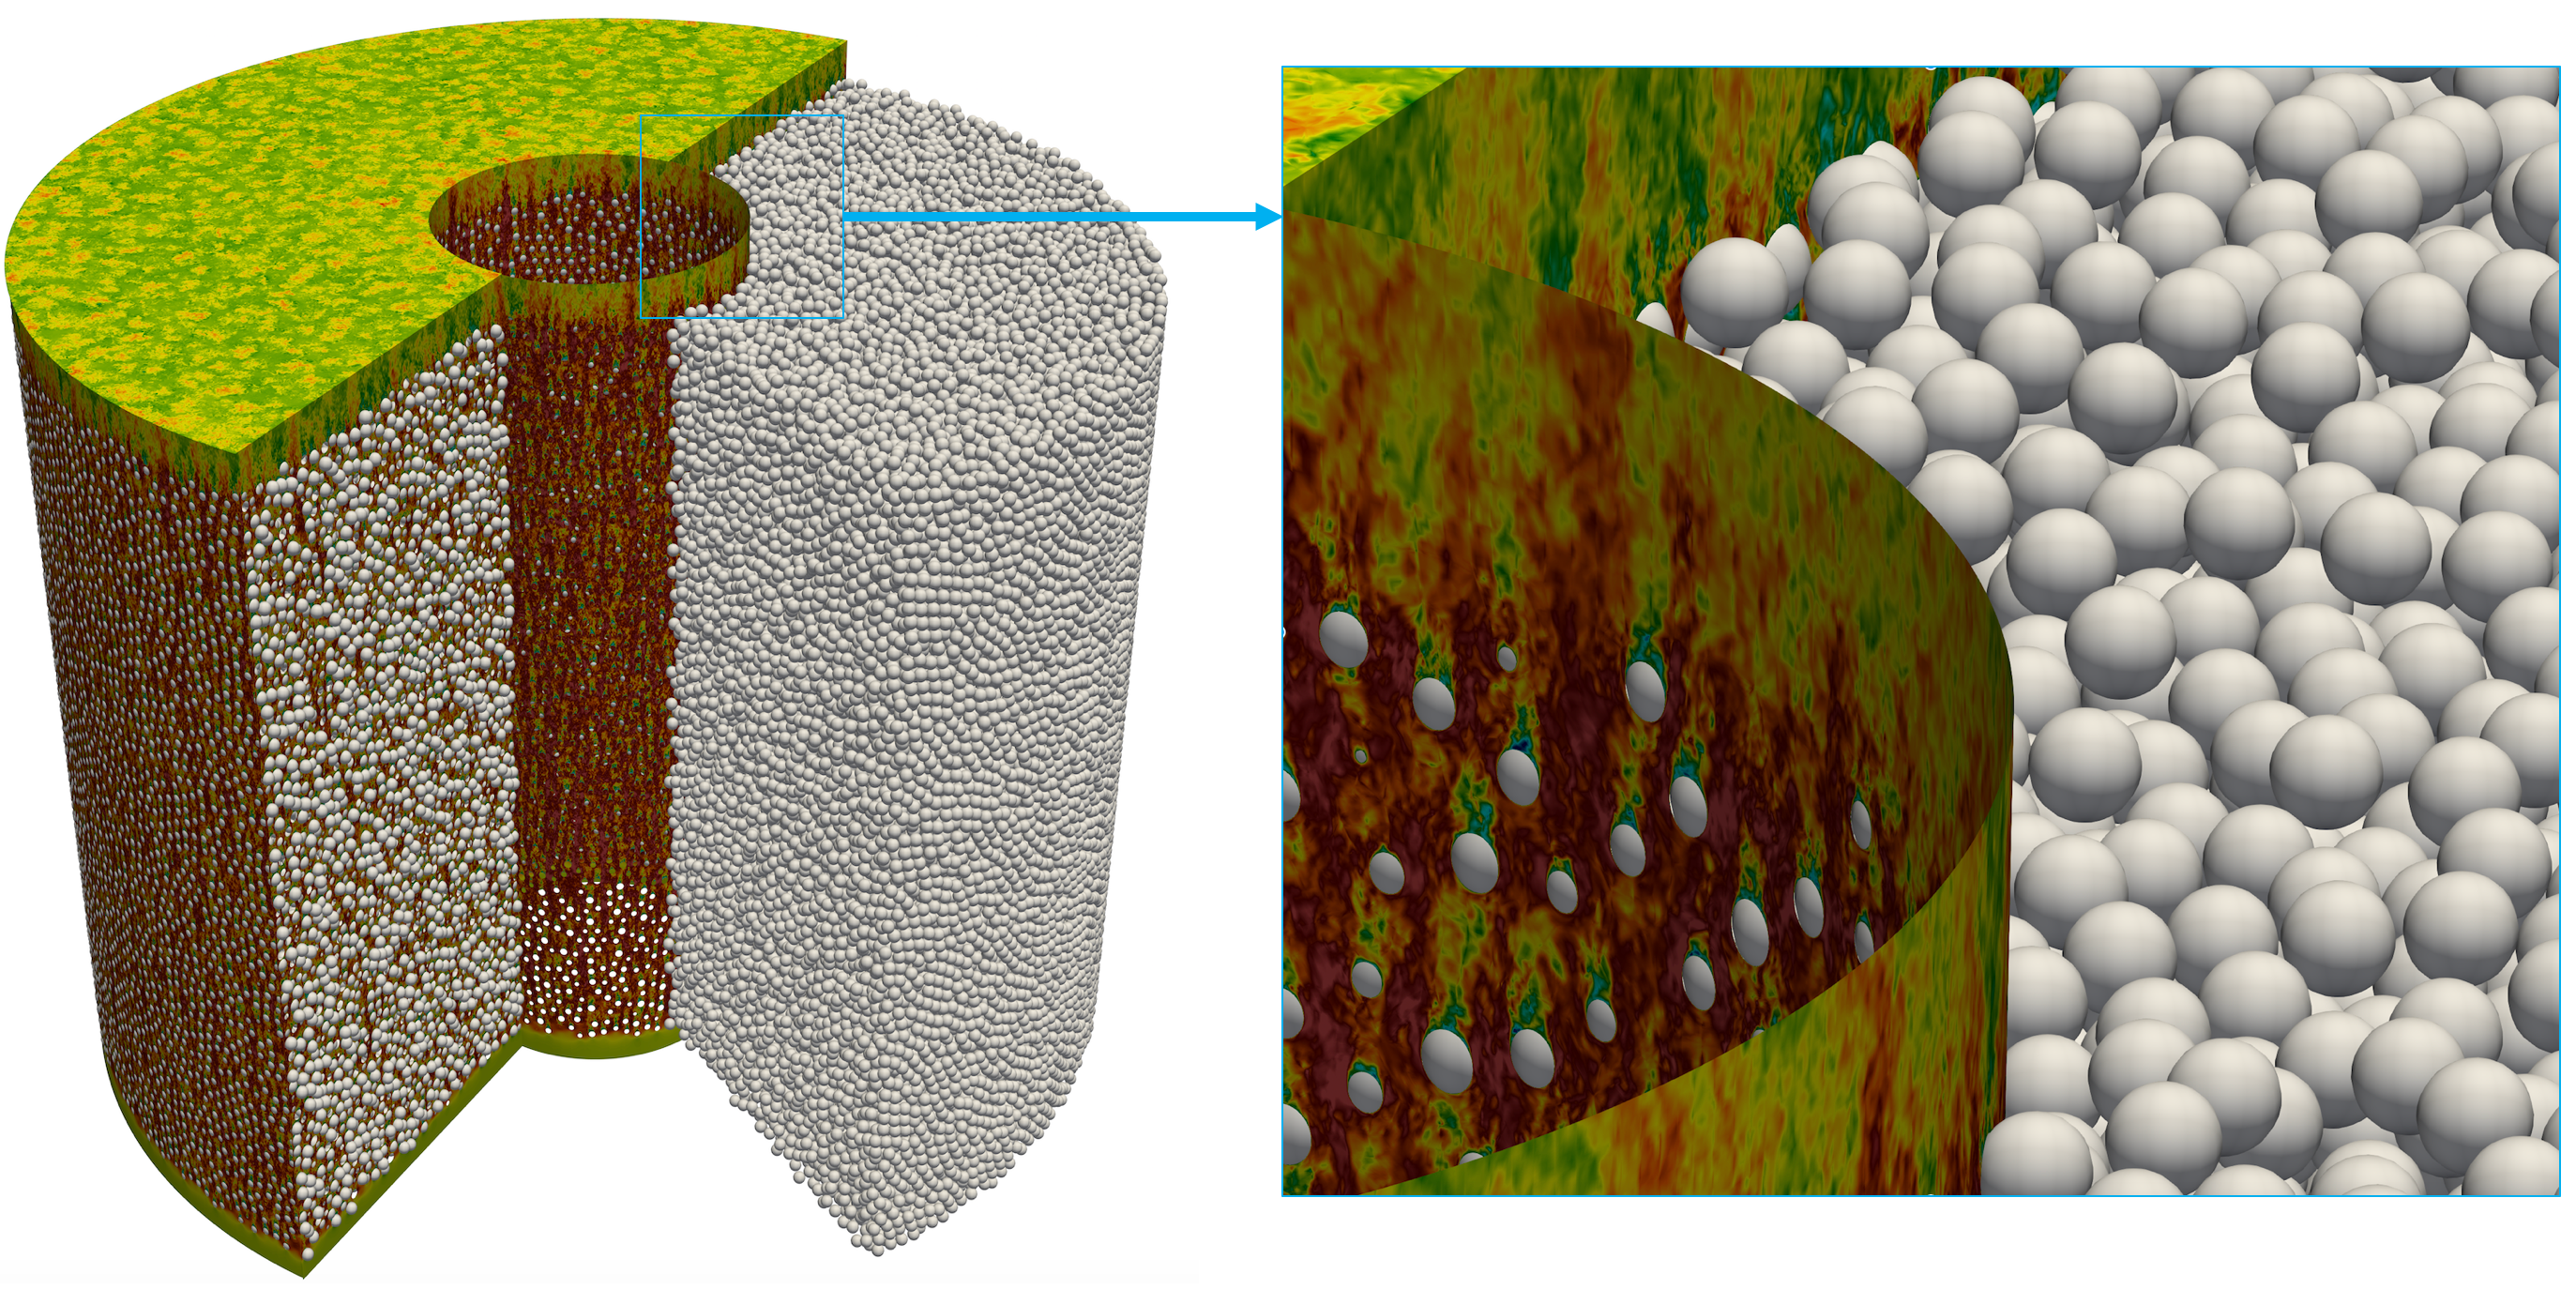
\includegraphics[width=0.93\textwidth]{figures/350K_peb.png}
 \caption{\label{fig:350k} Reactor simulations of turbulent flow performed 
  on OLCF/Summit:
  full core with 352,625 pebbles using an all-hex mesh comprising
  $E$=98,782,067 elements of order $N=8$.}
\end{figure}
%%%%%%%%%%%%%%%%%%%%%%%%%%%%%%%%%%%%%%%%%%%%%%%%%%%%%%%%%%%%%%%%%%%%%%%%%%


%%%%%%%%%%%%%%%%%%%%%%%%%%%%%%%%%%%%%%%%%%%%%%%%%%%%%%%%%%%%%%%%%%%%%%%%%%
\begin{table}
\footnotesize
\begin{center}
\begin{tabular}{|c|c|c|c|c|c|c|}
  \hline
  \multicolumn{7}{|c|}{{\bf NekRS Strong Scale: 352K pebbles, $E$=98M, $n$=50B}}\\
  \hline
% \multicolumn{7}{|c|}{Re=500, 2.e-3, 9, 13, 4.e-4, TOMBO2, 1, T, 8, F, CHEBY+JAC, 851}\\
  \multicolumn{7}{|c|}{{\bf $N=8$, $N_q=11$, $\Delta t=$ 8.e-4, $L=30$, 2-Cheb-ASM:8641}}\\
  \hline
  Node & GPU  & $n/P$ &  $v_i$ & $p_i$ & $t_{\rm step}$ & Eff \\
  \hline
  1536   &  9216  &   5.4M   &  -   &   -  &    -   &      -       \\% MEM GB  \\
  2304   &  13824 &   3.6M   &   5.7&   7.2&    .55 &    100       \\% 15.1    \\
  3072   &  18432 &   2.7M   &   5.7&   7.2&    .56 &    73.6      \\% 10.8    \\
  3840   &  23040 &   2.1M   &   5.7&   7.2&    .39 &    84.6      \\% 9.57    \\
  4608   &  27648 &   1.8M   &   5.7&   7.2&    .36 &    76.3      \\% 8.04    \\
 \hline
 \end{tabular}
\end{center}
 \caption{\label{peb35k-strong}
 NekRS Strong Scale using BDF2 with characteristic.}
\end{table}
%%%%%%%%%%%%%%%%%%%%%%%%%%%%%%%%%%%%%%%%%%%%%%%%%%%%%%%%%%%%%%%%%%%%%%%%%%




 %%%%%%%%%%%%%%%%%%%%%%%%%%%%%%%%%%%%%%%%%%%%%%%%%%%%%%%%%%%%%%%%%%%%%%%%%
 \begin{table*}[!h]
  \footnotesize
  \begin{center}
  \begin{tabular}{|l|c|c|c|c|c|}
  \hline
  \multicolumn{6}{|c|}{{\bf NekRS Single GPU Performance, $E=7168$, $N=7$, $n=2.4M$, $Re=5000$}} \\
  \hline
   system   &  backend &  $t_{500}$     &   $t_{100}$    &   $t_{step}$ & R \\
  \hline
    Summit/V100   &  CUDA   &    4.089e+01  &  9.018e+00 &  0.0795 & 1.00   \\
    ThetaGPU/A100 &  CUDA   &    2.503e+01  &  5.587e+00 &  0.0485 & 0.61   \\
    Spock/MI100   &  HIP    &    5.007e+01  &  1.103e+01 &  0.0975 & 1.22   \\
    Tulip/MI100   &  HIP    &    4.870e+01  &  1.060e+01 &  0.0953 & 1.19   \\
  \hline
  \end{tabular}
  \end{center}
  \caption{\label{tb:singlerod} NekRS performance on a single GPU.
   Simulations are performed for 500 steps and the averaged timing per step, $t_{step}$,
   is measured in seconds for 101-500 steps. R is the ratio of $t_{step}$ to Summit V100.
   Different versions of ROCm are used for MI100.
   The timestep size is $\Delta t$=1.2e-03 (CFL=7.3).
   Characteristic-based BDF2 with 1 substeps is used for timestepping.
   Tolerances for pressure and velocity are  1e-4 and 1e-6, respectively.}
 \end{table*}
%%%%%%%%%%%%%%%%%%%%%%%%%%%%%%%%%%%%%%%%%%%%%%%%%%%%%%%%%%%%%%%%%%%%%%%%%

